\documentclass{article}
\usepackage[utf8]{inputenc}
\usepackage[T1]{fontenc}
\usepackage{geometry}
\usepackage{graphicx}
\usepackage{fancyhdr}
\usepackage{lastpage}
\usepackage[french]{babel}
\usepackage{chngcntr}
\usepackage{subcaption} 
\usepackage{url}
\usepackage{tabularx}
\usepackage{amssymb}
\usepackage{amsmath}
\usepackage{multicol}
\counterwithin{figure}{subsection} % Remettre le compteur de figure à zéro à chaque section







\pagestyle{fancy}
\geometry{textwidth=15.5cm,headheight= 12.17pt, footskip=40.34pt}
\makeatletter\@removefromreset{footnote}{chapter}\makeatother
\cfoot{2022-2023}
\fancyfoot[R]{\thepage\ of \pageref{LastPage}}
\fancyfoot[L]{\raisebox{-0.8cm}[0pt][0pt]{
\includegraphics[scale=0.15]{lyon logo.png}}} % Descend le logo 
\lhead{\leftmark}
\rhead{}



\begin{document}
%Page de garde 
\thispagestyle{empty}
\fancyfoot[L]{\raisebox{-0.8cm}[0pt][0pt]{
\includegraphics[scale=0.15]{lyon logo.png}}} % Descend le logo 
\begin{center}
    {\Large{Université Claude Bernard}} \\\vfill
    \textsc{\huge{rapport d'étude}} \\
    \vfill
    {\Large{UE-PHY1188M Modélisation Numérique}}
    \vfill
    \rule{0.95\textwidth}{0.5pt}\\\vspace{0.9\baselineskip}

    {\Huge{\textbf{Etude du modèle d'Ising par simulation numérique sous C++}}} 
    \rule{0.95\textwidth}{0.5pt}\\\vfill
    {\Large{soutenu le 28 Avril 2023\\
    \vspace{1\baselineskip}
    par \\
    \vspace{1\baselineskip}
    LOQUET Antoine}} \\\vfill
\end{center}

\Large\emph{Encadrant :}\normalsize \\
\rule{0.42\textwidth}{0.1pt}\\
{\large{ALLOUCHE Abdul-Rahman}} \\

% Fin de Page de garde

\newpage

\vspace*{\fill}
\begin{center}
\tableofcontents
\end{center}
\vspace*{\fill}

\newpage


\section{Introduction}

Le modèle d'Ising est l'un des modèles les plus étudiés en physique statistique, en particulier en ce qui concerne la théorie des transitions de phase. Il a été introduit en 1925 par le physicien allemand Ernst Ising pour étudier la magnétisation de certains matériaux. Depuis lors, le modèle d'Ising est devenu un outil précieux pour étudier une grande variété de phénomènes physiques, allant des transitions de phase magnétiques aux propriétés de transport dans les matériaux désordonnés. Le modèle d'Ising est un système simplifié constitué de spins classiques, qui peuvent prendre les valeurs +1 ou -1, et qui sont disposés sur une grille de la dimension souhaitée\footnote{Dans le cas de ce rapport seules les dimensions deux et trois sont traitées}. Ces spins interagissent entre eux selon une certaine règle, ce qui donne lieu à des comportements collectifs émergents et à des transitions de phase intéressantes. Dans cette étude, nous allons explorer les principales caractéristiques du modèle d'Ising et discuter des résultats de la simulation. 

\section{Théorie}

Cette partie est consacrée à l'explication théorique des caractéristique du modèle d'Ising traité par le programme. Pour plus de détails, il faut consulter \cite{Phystat}. Le modèle d'Ising est à la base une version simplifiée du modèle d'Heisenberg sur le magnétisme. Ce dernier a mit en évidence à l'aide de l'antisymétrisation des fonctions d'onde électroniques due au principe d'exclusion de Pauli, le comportement ferromagnétique qui était jusqu'à lors un mystère. 


\subsection{Interaction d'échange entre deux spins}

L'argument d'Heisenberg est basé sur l'analyse d'un système de deux électrons et deux ions massifs que l'on suppose immobiles. Ainsi l'hamiltonien de ce système s'écrit : 
\begin{equation}
    H= h(1) + h(2) + \frac{e^2}{4\pi\epsilon_{0}r_{12}}
\end{equation}

où h(1) et h(2)  contiennent respectivement l'énergie cinétique ainsi que le potentiel d'interaction entre l'électron et les ions. $r_{12}$ quant à lui désigne la distance entre les deux électrons. Cependant l'argument du physicien repose sur l'hamiltonien réduit, ainsi le dernier terme disparaît. Si nous suivons le raisonnement de \cite{Phystat}, nous arrivons à l'hamiltonien suivant : 

\begin{equation}
   H=-J\sum_{\langle ij \rangle}^{}\sigma_{i}\sigma_{j}  - h\sum_{i}^{}\sigma_{i}
   \label{H}
\end{equation}

J représente l'intégrale d'échange entre les plus proches voisins. Si la constante J est positive, le matériau est ferromagnétique, ce qui veut dire que les spins tendent à s'aligner. À  l'inverse, si J est négative, les spins tendent à être antiparallèle, on parle alors de modèle antiferromagnétique. $\langle ij \rangle$ une somme sur les plus proches voisins et h un champ magnétique externe. Ce dernier tend à aligner les spins dans la même direction que  lui. De là dérive la formule permettant de calculer la différence d'énergie engendrée par le renversement d'un spin (formule \ref{deltaE}). $\sigma_{i \ et  \ j}$ représentent le spin d'un site.

\subsection{Formules principales}

Depuis la formule \ref{H}, on peut calculer la relation suivante :
\begin{equation}
    \Delta E=2S(h+J\sum_{\langle ij \rangle}^{4  \ ou \ 6}S_{premiers \ voisins})
    \label{deltaE}
\end{equation}

S représente le spin du site ij tiré au hasard. $S_{premiers \ voisins}$ correspond au spin d'un premier voisin. Concernant la somme elle varie entre quatre et six selon la dimension. En effet si la dimension du système est deux alors le site ij à quatre premiers voisins, et six si la dimension est trois. \\

La susceptibilité magnétique $\chi_m$ mesure la capacité d'un matériau à devenir magnétique en présence d'un champ magnétique externe. La formule dont se sert la simulation pour la calculer est la formule \ref{Xi}, avec M qui représente la magnétisation moyenne. La formule a été donnée et non démontrée dans \cite{Simu}.


\begin{multicols}{2}
\noindent 
\begin{equation}
    \chi_m = \frac{\left\langle M^2 \right\rangle-\left\langle M\right\rangle^2}{k_{b}T}
    \label{Xi}
\end{equation} 
\begin{equation}
   M=\frac{1}{N}\sum_{i}^{N}\sigma_{i}
   \label{Mag}
\end{equation} 
\end{multicols} 

Avec N qui représente le nombre de spin total. Une autre manière de calculer la magnétisation moyenne est donnée par la solution analytique au modèle d'Ising dans la limite thermodynamique a été fournie par Lars Onsager en 1944 : 

\begin{equation}
\left\langle M \right\rangle(T)= \left\{
\begin{array}{ll}
\left( 1-\sinh\left(\frac{2J}{k_{b}T}\right)^{-4} \right)^{1/8} & \mbox{si } T<T_{c} \\
0 & \mbox{sinon} 
\end{array}
\right.
\label{Magtheo}
\end{equation}

Ainsi pour déterminer la température critique théorique du système, il suffit de déterminer pour quelle température la magnétisation moyenne s'annule en fonction de son intégrale d'échange. La dernière formule utilisée dans la simulation est celle de la capacité volumique, notée $C_{v}$ (formule \ref{Cv}). Cette notion caractérise la quantité de chaleur nécessaire pour modifier d'une unité la température d'un matériau sans changer ses conditions externes. 

\begin{equation}
    C_{v} = \frac{\left\langle E^2 \right\rangle-\left\langle E\right\rangle^2}{(k_{b}T)^2}
    \label{Cv}
\end{equation} 

avec E l'énergie du système. 
\section{Algorithme}

Afin de traiter au mieux ce modèle théorique, j'ai réalisé une simulation numérique. Ainsi dans cette section, je vais détailler mon programme. \\

Il arrive que les programmes se retrouvent dans une file d'attente pour être effectués. Il est alors judicieux de placer les variables nécessaires dans une fichier à part. En effet, si l'on s'aperçoit que les données ne sont pas correctes, ou bien que l'on veut simplement les modifier, cela n'est possible que par le biais de cette méthode. C'est dans cet objectif que la simulation de mon projet commence. \\

Dans ce fichier texte, on y retrouve par exemple la valeur de l'intégrale d'échange, la dimension de la simulation, la taille du système, les variables de températures, etc. Une fois les variables allouées dans le programme, ce dernier affiche la température critique théorique, puis appelle la fonction \emph{Simulation}. Cette dernière est le cœur de la simulation est voici comment elle fonctionne : \\

Tout d'abord, la fonction agit en fonction de la dimension du système sélectionnée dans le fichier texte. Dans une optique de non-répétition seule la dimension deux sera expliquée dans ce rapport. Dans les faits, la dimension trois ressemble à quelques détails près à cette dernière. 

Un site ij est tiré aléatoirement dans le système. À l'aide de la fonction \emph{PremierVoisin}, les spins des quatre premiers voisins du site sont sommés. Cette dernière prend en compte les effets de bord. Cela se traduit par une duplication du système, puis une juxtaposition de cette dernière à côté du site ij lorsqu'il est tiré sur un bord de la grille. Cet effet permet d'éviter que le site ne possède que deux ou trois voisins selon s'il est tiré dans un coin ou une bordure de grille. Dès lors, le programme calcule la différence d'énergie due au changement de spin à l'aide de la relation (\ref{deltaE}). Si la différence est négative, le spin est inversé, autrement un nombre aléatoire est tiré entre 0 et 1. Si $e^{-\frac{\Delta E}{k_{b}T}}$ est inférieure à ce dernier, le spin est inversé. Dans n'importe quelle autre situation, aucun changement est effectué. Si le spin a été inversé, la différence d'énergie est alors additionnée à l'énergie initialement nulle. La partie sur la décision de changement de spin s'appelle l'algorithme de Métropolis.\\

Dans le but de calculer $C_{v}$, la simulation somme toutes les énergies et les énergies au carré auxquelles elle retranchera le nombre d'itérations effectuées, afin d'appliquer la formule (\ref{Cv}). Effectivement, le tirage aléatoire d'un site ij, le calcul de la différence d'énergie, et l'algorithme de Métropolis sont répétés autant de fois que l'utilisateur le souhaite\footnote{À noter que pour une simulation représentative, un nombre d'itérations important est requit. Pour ma part je faisais 1 million d'itérations}. Pour finir, toutes ces étapes sont bouclées sur plage de température et un pas de température définit dans le fichier texte. \\

Concernant la magnétisation et la susceptibilité magnétique, à chaque température la fonction \emph{Simulation} initialise une variable \textbf{mag} avec la fonction \emph{magnetisation}. Cette dernière a pour objectif de calculer la somme de tous les spins de la grille. Lorsqu'un spin est renversé, le programme ajoute deux fois la valeur du nouveau spin à \textbf{mag}. Ainsi à l'instar de la méthode pour calculer $C_{v}$, le programme calcule la magnétisation et les magnétisations au carré auxquelles il retranchera le nombre d'itérations effectuées. Cependant, il est nécessaire de tenir compte de la taille de la grille pour avoir une aimantation moyenne. C'est pourquoi la magnétisation est divisée par la taille du système en plus du nombre d'itérations pour chaque température. La susceptibilité magnétique est calculée à l'aide de la relation \ref{Mag} pour chaque température. \\

Afin d'analyser les résultats, ces derniers sont enregistrés dans deux fichiers textes différents. Dans le premier se trouvent en première colonne les températures, puis les différents $C_{v}$ et pour finir les énergies. Le second fichier enregistre quant à lui les différents $\chi_m$ à la place des $C_{v}$ et la magnétisation moyenne à la place de l'énergie. \\

Le programme peut si demandé par l'utilisateur, enregistrer dans un fichier texte la grille à la température désirée. Dans la première colonne sont notés les i, puis dans la deuxième les j et la troisième les valeurs. Cela permettra de mettre en évidence plusieurs comportements caractéristique du modèle d'Ising. 

\section{Résultats}

Lors de cette section, toutes les courbes, tous les graphiques sont tracés à l'aide de Python depuis les fichiers textes enregistrés lors de la simulation. De plus, afin d'analyser les résultats, je me suis permis de faire du traitement de données dans certains cas sous Python également.


\subsection{Énergie et Capacité calorifique}
\label{subsec:Energie et CV}

Dans cette sous-section le champ magnétique externe est nul, l'intégrale d'échange \emph{J} est égale à 1e-21J, ce qui donne une température critique égale à 164.356K. Afin de mettre en évidence cette température critique, il suffit de tracer $C_{v}$ en fonction de la température. On obtient donc un pic caractéristique aussi bien sur la simulation 2D que 3D, visibles à l'aide des figures \ref{Tc_2D} et \ref{Tc_3D}. On détermine la température critique du modèle 2D à 165K. On constate que la température critique du modèle 3D diffèrent de 154K. Seule la simulation 2D donne un résultat acceptable pour la valeur de $T_{c}$. Cependant pour améliorer la précision du résultat, il est possible diminuer le pas de variation de température ce qui ne sera pas fait dans ce rapport. 


\begin{figure}[ht]
  \centering
  \begin{minipage}[b]{0.45\textwidth}
    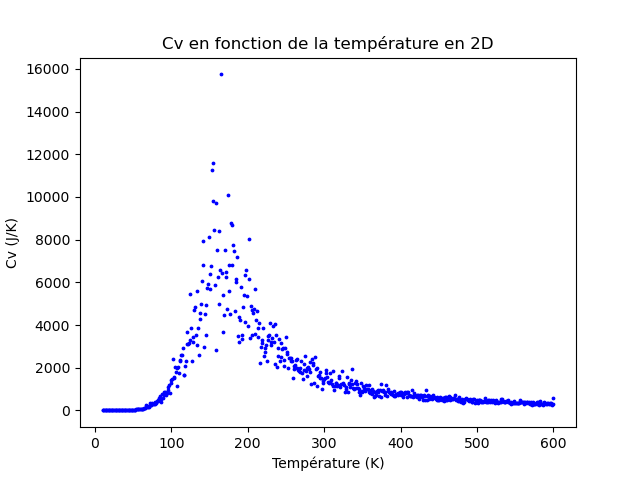
\includegraphics[height=5.5cm]{Tc/Tc en 2D.png}
    \caption{Température critique = 165K}
    \label{Tc_2D}
  \end{minipage}
  \hspace{0.5cm}
  \begin{minipage}[b]{0.45\textwidth}
    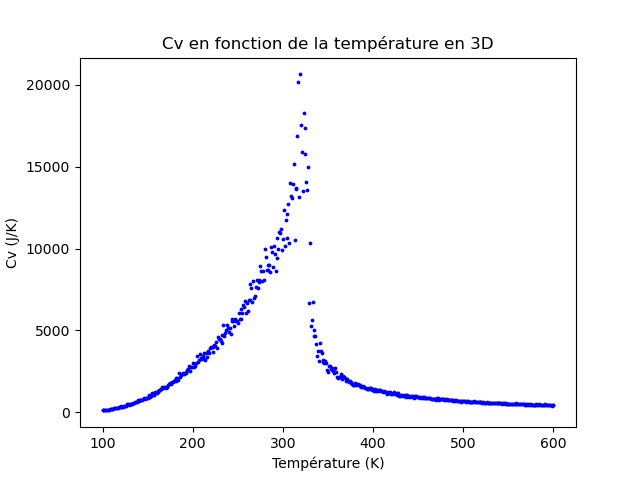
\includegraphics[height=5.5cm]{Tc/Tc_en_3D.png}
    \caption{Température critique = 319K}
    \label{Tc_3D}
  \end{minipage}
\end{figure}

De plus, on peut mettre en évidence la variation de l'énergie d'un système en fonction de la température (figure \ref{energie}). On aperçoit à la température critique une nette variation de l'énergie du système, jusqu'à tendre vers 0. Cela se traduit par une incapacité à changer d'état dans la grille et une atteinte d'un état d'équilibre.  

\begin{figure}[ht]
  \centering
  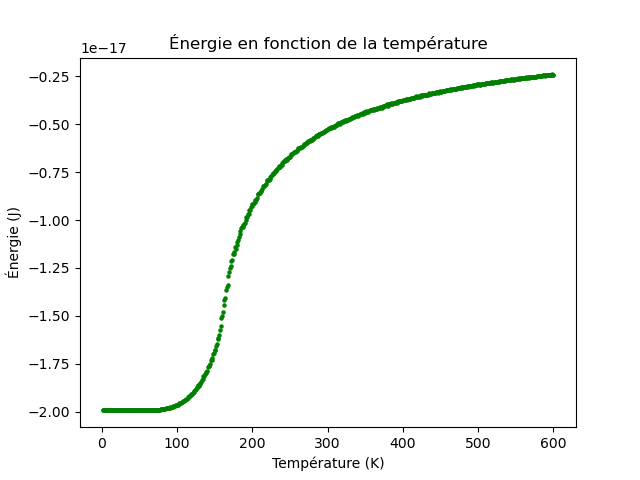
\includegraphics[height=5.5cm]{Tc/Energie plot.png}
  \caption{Variation de l'énergie en fonction de la température pour un modèle 2D}
  \label{energie}
\end{figure}


\newpage
\subsection{Domaines de Weiss}

Les paramètres de simulations restent inchangés par rapport à la sous-section \ref{subsec:Energie et CV}. L'objectif de cette sous-section est de montrer les grilles avant et après la température critique. \\

Depuis la sous-section précédente, nous savons que la température de transition du système 2D est de 165K et de 319K pour le 3D. Ainsi, dans le fichier variables.txt, les températures d'affichages ont été définies à 10K et 500K pour être en dessous et au dessus des deux $T_{c}$.

\begin{figure}[htbp]
  \centering
  \begin{subfigure}[b]{0.22\textwidth}
    \centering
    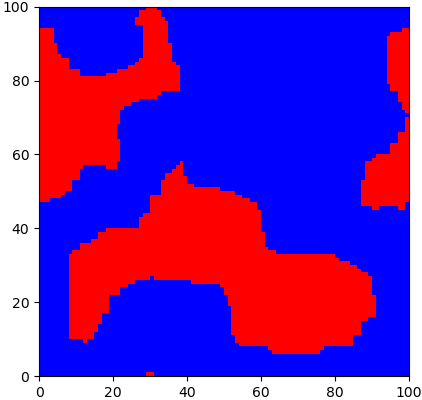
\includegraphics[width=\textwidth]{DW/Grille_cut_10K_V2.png}
    \caption{Température 10K}
    \label{2D_10K}
  \end{subfigure}\hfill
  \begin{subfigure}[b]{0.22\textwidth}
    \centering
    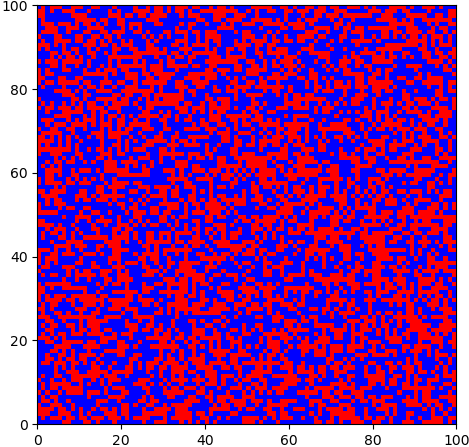
\includegraphics[width=\textwidth]{DW/Grille_cut_500K_V2.png}
    \caption{Température 500K}
    \label{2D_500K}
  \end{subfigure}\hfill
  \begin{subfigure}[b]{0.22\textwidth}
    \centering
    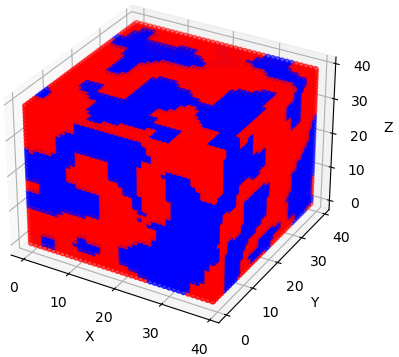
\includegraphics[width=\textwidth]{DW/Grille_3D_cut_10K.png}
    \caption{Température 10K}
    \label{3D_10K}
  \end{subfigure}\hfill
  \begin{subfigure}[b]{0.22\textwidth}
    \centering
    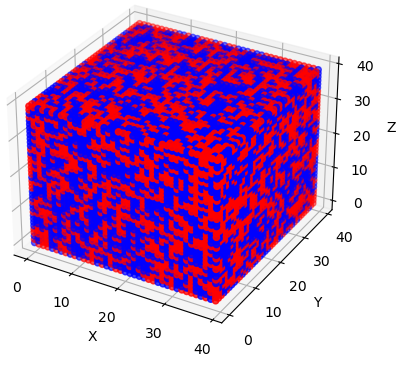
\includegraphics[width=\textwidth]{DW/Grille3D_500K.png}
    \caption{Température 500K}
    \label{3D_500}
  \end{subfigure}
  
  \caption{Représentation de la matrice du système de dimension deux ((a) et (b)) ainsi que la dimension trois ((c) et (d)). La couleur rouge correspond à un spin de valeur +1, et la bleue à un spin de valeur -1}
  \label{4TC}
\end{figure}

Sur les deux dimensions de la figure \ref{4TC}, nous constatons qu'il y a une transition de phases entre les deux températures. En effet, sur les figures \ref{2D_10K} et \ref{3D_10K}, on visualise nettement des domaines  dans lesquelles les moments magnétiques s'alignent entre eux. On appelle ces domaines de Weiss. Et sur les figures \ref{2D_500K} et \ref{3D_500} une homogénéisation de la répartition de l'orientation des spins. Cela se traduit par une perte des propriétés magnétiques du réseau. Les domaines de Weiss quant à eux mettent en évidence l'aimantation spontanée du réseau.

\subsection{Magnétisation moyenne et susceptibilité magnétique}

Une autre manière de voir les propriétés magnétiques de la grille est d'afficher la magnétisation ainsi que la susceptibilité magnétique en fonction de la température. De plus, d'après la formule \ref{Magtheo} il est possible de connaître la forme théorique de la magnétisation en fonction de la température. 

\begin{figure}[ht]
  \centering
  \begin{minipage}[b]{0.45\textwidth}
    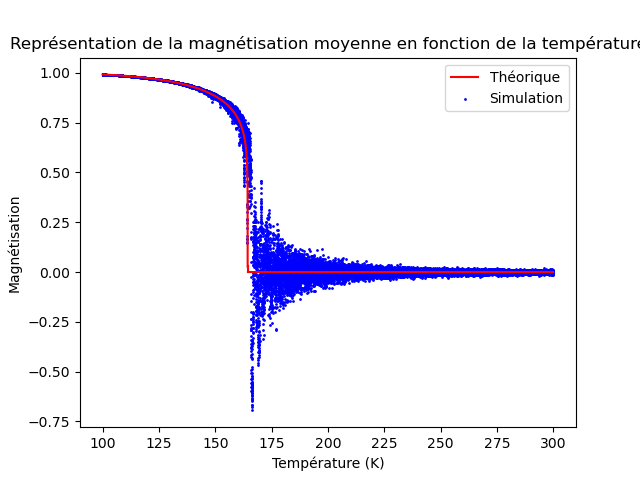
\includegraphics[height=5.5cm]{Mag/Magnétisation en fonction de T.png}
    \caption{Température critique = 165K}
    \label{Mag_2D}
  \end{minipage}
  \hspace{0.5cm}
  \begin{minipage}[b]{0.45\textwidth}
    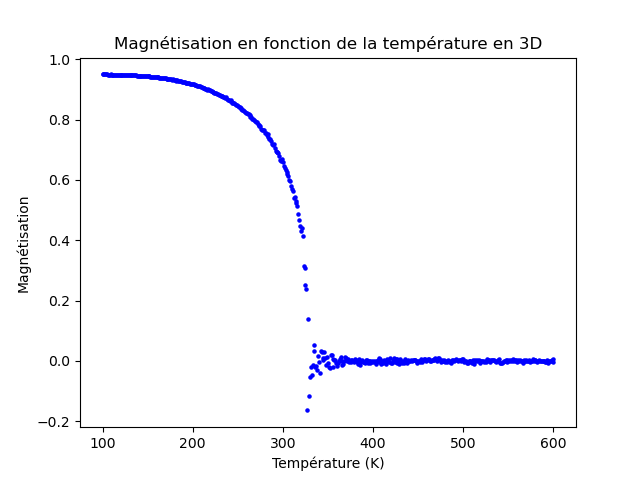
\includegraphics[height=5.5cm]{Mag/Mag_en_3D.png}
    \caption{Température critique = 319K}
    \label{Mag_3D}
  \end{minipage}
\end{figure}

Sur les figures \ref{Mag_2D} et \ref{Mag_3D} on retrouve, les valeurs des températures critiques pour les modèles 2D et 3D lorsque la magnétisation tombe à 0. La figure \ref{Mag_2D}, nous permet de dire que la simulation 2D et la théorie concordent. Cependant on remarque des fluctuations plus ou moins importantes après la température jusqu'à tendre vers 0. Ces fluctuations sont dues à la partie aléatoire de la simulation. Il est possible de réduire ces fluctuations en augmentant les itérations ce qui permet d'avoir les fluctuations de la figure \ref{Mag_3D}. \\

À  l'instar de la capacité calorifique, nous pouvons tracer la susceptibilité magnétique en fonction de la température. 

\begin{figure}[ht]
  \centering
  \begin{minipage}[b]{0.45\textwidth}
    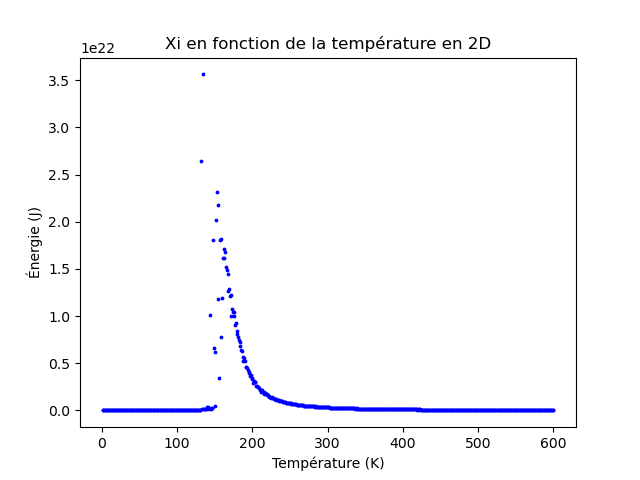
\includegraphics[height=5.5cm]{Mag/Xi_en_2D.png}
    \caption{Température critique = 165K}
    \label{Xi_2D}
  \end{minipage}
  \hspace{0.5cm}
  \begin{minipage}[b]{0.45\textwidth}
    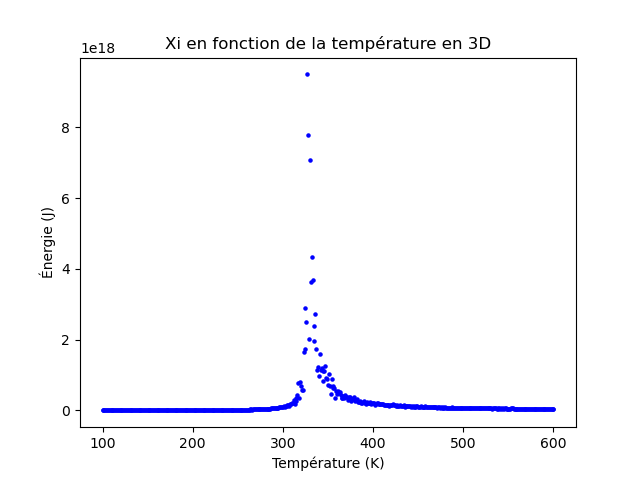
\includegraphics[height=5.5cm]{Mag/Xi_en_3D.png}
    \caption{Température critique = 319K}
    \label{Xi_3D}
  \end{minipage}
\end{figure}

On constate que les figures \ref{Xi_2D} et \ref{Xi_3D}, nous donnent respectivement une température critique de 165K et 319K pour les simulations. Ces températures critiques sont déterminée au maximum d'énergie. Ces résultats restent en accord avec les précédents. 

\subsection{Évolution de la température critique en fonction de la taille du système ou d'un champ magnétique externe}

Jusqu'à lors dans les simulations les paramètres restaient identiques. Au sein de cette sous-section, nous allons faire varier un premier paramètre, la taille du système (figure \ref{Var_taille}), puis nous allons voir l'effet d'un champ magnétique externe sur la grille (figure \ref{CvB}).




\begin{figure}[htbp]
  \centering
  \begin{minipage}[b]{0.45\textwidth}
    \centering
    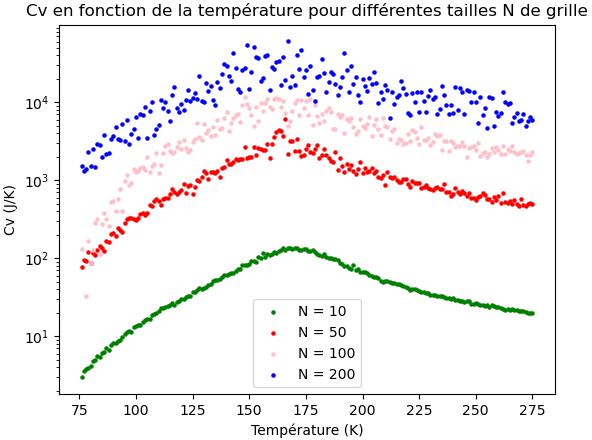
\includegraphics[scale=0.65]{Cv_en_fonction_de_la_taille.png}
    \caption{Le graphique est zoomé sur la zone d'intérêt. L'axe des $C_{v}$ est en échelle logarithmique pour visualiser correctement toutes les variations.}
    \label{Var_taille}
  \end{minipage}
    \hspace{0.2cm}
      \raisebox{2cm}{%
  \begin{minipage}[b]{0.4\textwidth}
    \centering
    \begin{tabular}{cclll}
    \cline{1-2}
    \multicolumn{1}{|c|}{\textbf{Taille du système}} & \multicolumn{1}{c|}{\textbf{Température critique}} &  &  &  \\ \cline{1-2}
   \multicolumn{1}{|c|}{10}                         & \multicolumn{1}{c|}{168 K}                         &  &  &  \\ \cline{1-2}
    \multicolumn{1}{|c|}{50}                         & \multicolumn{1}{c|}{164 K}                         &  &  &  \\ \cline{1-2}
     \multicolumn{1}{|c|}{100}                        & \multicolumn{1}{c|}{165 K}                         &  &  &  \\ \cline{1-2}
      \multicolumn{1}{|c|}{200}                        & \multicolumn{1}{c|}{161 K}                         &  &  &  \\ \cline{1-2}
     \multicolumn{1}{l}{}                             & \multicolumn{1}{l}{}                               &  &  & 
     \end{tabular}
    \captionof{table}{Tableau résumant les températures critiques en fonction de la taille du système}
    \label{Tab_taille}
  \end{minipage}%
  }
\end{figure}

À l'aide du tableau \ref{Tab_taille}, on ne voit pas de changement significatif de température critique comparé à la valeur théorique. Cela est dû à la condition de bord périodique. Concernant la variation de $T_{c}$ en fonction d'un champ magnétique externe h, la figure \ref{CvB} met en évidence un décalage de la température critique vers de plus hautes températures. L'élévation de la température tend à perturber la stabilité de l'orientation des spins, mais le fait que le champ h impose une orientation, cela permet de lutter contre. De plus, on remarque facilement que caractériser les températures critiques de la courbe rose et bleue n'est plus possible en sélectionnant seulement le maximum. C'est pourquoi j'ai lissé les valeurs sur une fenêtre de 47 points. Néanmoins le lissage n'est pas suffisant pour trouver le centre des deux courbes précédemment citées. Dans un objectif de ne pas trop dégrader les données, j'ai réalisé un fitting d'une parabole (figure \ref{CvB_liné}).

\begin{figure}[htb]
  \centering
  \begin{minipage}[t]{0.45\textwidth}
    \vspace{0pt}
    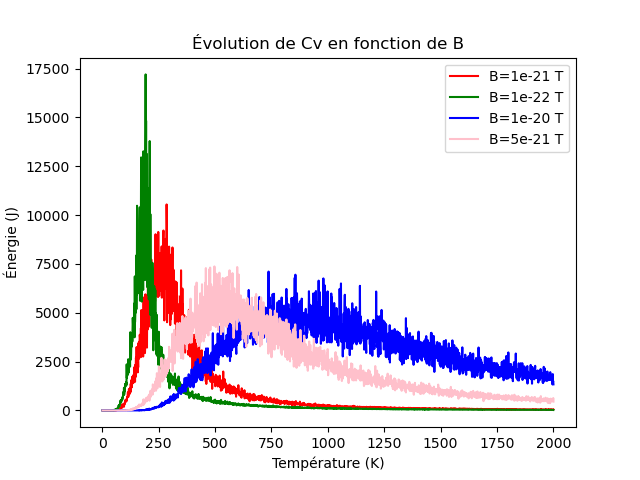
\includegraphics[height=5.5cm]{VarB/Variation_de_Tc_en_fonction_de_B_cut.png}
    \caption{Chaque courbe représente l'évolution de $C_{v}$ en fonction de la température avec un champ magnétique externe associé.}
    \label{CvB}
  \end{minipage}
  \hspace{0.5cm}
  \begin{minipage}[t]{0.45\textwidth}
    \vspace{0pt}
    \includegraphics[height=5.5cm]{VarB/Cv_linéarisées_(N={N})_en_fonction_de_B.png}
    \caption{Linéarisation sur 47 points et fitting de courbes.}
    \label{CvB_liné}
  \end{minipage}
\end{figure}

\newpage

En cherchant la position des maximums des courbes, on peut établir le tableau \ref{tablis}.

\begin{table}[h]
\centering
\begin{tabular}{|c|c|c|}
\hline
\begin{tabular}[c]{@{}c@{}}Champ magnétique\\  externe h (T)\end{tabular} & \begin{tabular}[c]{@{}c@{}}Température (K) des \\ courbes non lisées\end{tabular} & \begin{tabular}[c]{@{}c@{}}Température (K) des \\ courbes lisées\end{tabular} \\ \hline
h= 1e-22                                                                  & 192                                                                               & 188                                                                           \\ \hline
h= 1e-21                                                                  & 285                                                                               & 268                                                                           \\ \hline
h= 5e-21                                                                  & 497                                                                               & 538                                                                           \\ \hline
h=1e-20                                                                   & 737                                                                               & 949                                                                           \\ \hline
\end{tabular}
\caption{Tableau comparant les températures critiques en fonction du lissage ou non.}
\label{tablis}
\end{table}

Ce dernier confirme bien le décalage de la température critique en fonction de h. De plus on constate graphiquement que les valeurs de $T_{c}$ pour les courbes lissées correspondent davantage que les non lissées. 


\section{Conclusion}

Par le biais de la simulation numérique, j'ai testé le modèle d'Ising en 2D et en 3D. L'étude de la simulation peut être approfondie en regardant l'importance du nombre d'itérations pour une température, ou bien regarder comment réagit le système si les conditions de bords périodiques sont annulées. Le modèle quant à lui peut être également amélioré en différenciant les intégrales d'échanges selon i ou j ou z selon la dimension, inclure l'action des deuxièmes plus proches voisins. Cependant, par souci de temps ces notions n'ont pas été étudiées. Néanmoins nous avons remarqué que les résultats concordaient avec la théorie. De plus, les résultats obtenus sont cohérents avec des simulations autre que la mienne tels que les références \cite{Simu}, \cite{Obs}. La rapidité de mon programme et la cohérence des résultats font de ce dernier un moyen correct pour exploiter dans une certaine mesure le modèle d'Ising.


\newpage
\begin{thebibliography}{99}
\bibitem{Phystat}   
Biben Thierry, \emph{Physique Statistiques des milieux en interactions}, [fichier PDF], Université Claude Bernard, 15 janvier 2019.

\bibitem{Simu} 
Roussel, Jimmy. \emph{Modèle d’Ising 2D}. 22 juin 2015, \url{https://femto-physique.fr/simulations/ising2D.php}.

\bibitem{Obs}
\emph{Simulation du modèle d’Ising}. \url{https://media4.obspm.fr/public/M2R/appliquettes/ising/doc/Ising_doc.html}.


\bibitem{Detail}
\emph{Modélisations et Simulations Modèle d'Ising}, [fichier PDF]. (s. d.). Detail-Ising.

\bibitem{Ising}
\emph{Modèle d'Ising},  [fichier PDF]. (s. d.). Modèle d’Ising.

\bibitem{Proj}
\emph{Projets d’informatique},[fichier PDF]. (s. d.). ListeProjetsM1.


\end{thebibliography}

\end{document}